%%%%%%%%%%%%%%%%%%%%%%%%%%%%%%%%%%%%%%%%%
% The Legrand Orange Book
% LaTeX Template
% Version 1.3 (21/8/13)
%
% This template has been downloaded from:
% http://www.LaTeXTemplates.com
%
% Original author:
% Mathias Legrand (legrand.mathias@gmail.com)
%
% License:
% CC BY-NC-SA 3.0 (http://creativecommons.org/licenses/by-nc-sa/3.0/)
%
% Compiling this template:
% This template uses biber for its bibliography and makeindex for its index.
% When you first open the template, compile it from the command line with the 
% commands below to make sure your LaTeX distribution is configured correctly:
%
% 1) pdflatex main
% 2) makeindex main.idx -s StyleInd.ist
% 3) biber main
% 4) pdflatex main x 2
%
% After this, when you wish to update the bibliography/index use the appropriate
% command above and make sure to compile with pdflatex several times 
% afterwards to propagate your changes to the document.
%
% This template also uses a number of packages which may need to be
% updated to the newest versions for the template to compile. It is strongly
% recommended you update your LaTeX distribution if you have any
% compilation errors.
%
% Important note:
% Chapter heading images should have a 2:1 width:height ratio,
% e.g. 920px width and 460px height.
%
%%%%%%%%%%%%%%%%%%%%%%%%%%%%%%%%%%%%%%%%%

%----------------------------------------------------------------------------------------
%	PACKAGES AND OTHER DOCUMENT CONFIGURATIONS
%----------------------------------------------------------------------------------------

\documentclass[11pt,fleqn,openany]{book} % Default font size and left-justified equations

\usepackage[top=3cm,bottom=3cm,left=3.2cm,right=3.2cm,headsep=10pt,a4paper]{geometry} % Page margins

\usepackage{xcolor} % Required for specifying colors by name
\definecolor{ocre}{RGB}{243,102,25} % Define the orange color used for highlighting throughout the book

\newcommand{\degree}{\ensuremath{^\circ}}
\usepackage{wrapfig}

% Font Settings
\usepackage{avant} % Use the Avantgarde font for headings
%\usepackage{times} % Use the Times font for headings
\usepackage{mathptmx} % Use the Adobe Times Roman as the default text font together with math symbols from the Sym­bol, Chancery and Com­puter Modern fonts

\usepackage{microtype} % Slightly tweak font spacing for aesthetics
\usepackage[utf8]{inputenc} % Required for including letters with accents
\usepackage[T1]{fontenc} % Use 8-bit encoding that has 256 glyphs

% Bibliography
\usepackage[style=alphabetic,sorting=nyt,sortcites=true,autopunct=true,babel=hyphen,hyperref=true,abbreviate=false,backref=true,backend=biber]{biblatex}
\addbibresource{bibliography.bib} % BibTeX bibliography file
\defbibheading{bibempty}{}

% Index
\usepackage{calc} % For simpler calculation - used for spacing the index letter headings correctly
\usepackage{makeidx} % Required to make an index
\makeindex % Tells LaTeX to create the files required for indexing

%----------------------------------------------------------------------------------------

%----------------------------------------------------------------------------------------
%	VARIOUS REQUIRED PACKAGES
%----------------------------------------------------------------------------------------

\usepackage{titlesec} % Allows customization of titles

\usepackage{graphicx} % Required for including pictures
\graphicspath{{img/}} % Specifies the directory where pictures are stored

\usepackage{lipsum} % Inserts dummy text

\usepackage{tikz} % Required for drawing custom shapes

\usepackage[english]{babel} % English language/hyphenation

\usepackage{enumitem} % Customize lists
\setlist{nolistsep} % Reduce spacing between bullet points and numbered lists

\usepackage{booktabs} % Required for nicer horizontal rules in tables

\usepackage{eso-pic} % Required for specifying an image background in the title page

%----------------------------------------------------------------------------------------
%	MAIN TABLE OF CONTENTS
%----------------------------------------------------------------------------------------

\usepackage{titletoc} % Required for manipulating the table of contents

\contentsmargin{0cm} % Removes the default margin
% Chapter text styling
\titlecontents{chapter}[1.25cm] % Indentation
{\addvspace{15pt}\large\sffamily\bfseries} % Spacing and font options for chapters
{\color{ocre!60}\contentslabel[\Large\thecontentslabel]{1.25cm}\color{ocre}} % Chapter number
{}  
{\color{ocre!60}\normalsize\sffamily\bfseries\;\titlerule*[.5pc]{.}\;\thecontentspage} % Page number
% Section text styling
\titlecontents{section}[1.25cm] % Indentation
{\addvspace{5pt}\sffamily\bfseries} % Spacing and font options for sections
{\contentslabel[\thecontentslabel]{1.25cm}} % Section number
{}
{\sffamily\hfill\color{black}\thecontentspage} % Page number
[]
% Subsection text styling
\titlecontents{subsection}[1.25cm] % Indentation
{\addvspace{1pt}\sffamily\small} % Spacing and font options for subsections
{\contentslabel[\thecontentslabel]{1.25cm}} % Subsection number
{}
{\sffamily\;\titlerule*[.5pc]{.}\;\thecontentspage} % Page number
[] 

%----------------------------------------------------------------------------------------
%	MINI TABLE OF CONTENTS IN CHAPTER HEADS
%----------------------------------------------------------------------------------------

% Section text styling
\titlecontents{lsection}[0em] % Indendating
{\footnotesize\sffamily} % Font settings
{}
{}
{}

% Subsection text styling
\titlecontents{lsubsection}[.5em] % Indentation
{\normalfont\footnotesize\sffamily} % Font settings
{}
{}
{}
 
%----------------------------------------------------------------------------------------
%	PAGE HEADERS
%----------------------------------------------------------------------------------------

\usepackage{fancyhdr} % Required for header and footer configuration

\pagestyle{fancy}
\renewcommand{\chaptermark}[1]{\markboth{\sffamily\normalsize\bfseries #1}{}} % Chapter text font settings
\renewcommand{\sectionmark}[1]{\markright{\sffamily\normalsize\thesection\hspace{5pt}#1}{}} % Section text font settings
\fancyhf{} \fancyhead[LE,RO]{\sffamily\normalsize\thepage} % Font setting for the page number in the header
\fancyhead[LO]{\rightmark} % Print the nearest section name on the left side of odd pages
\fancyhead[RE]{\leftmark} % Print the current chapter name on the right side of even pages
\renewcommand{\headrulewidth}{0.5pt} % Width of the rule under the header
\addtolength{\headheight}{2.5pt} % Increase the spacing around the header slightly
\renewcommand{\footrulewidth}{0pt} % Removes the rule in the footer
\fancypagestyle{plain}{\fancyhead{}\renewcommand{\headrulewidth}{0pt}} % Style for when a plain pagestyle is specified

% Removes the header from odd empty pages at the end of chapters
\makeatletter
\renewcommand{\cleardoublepage}{
\clearpage\ifodd\c@page\else
\hbox{}
\vspace*{\fill}
\thispagestyle{empty}
\newpage
\fi}

%----------------------------------------------------------------------------------------
%	THEOREM STYLES
%----------------------------------------------------------------------------------------

\usepackage{amsmath,amsfonts,amssymb,amsthm} % For including math equations, theorems, symbols, etc

\newcommand{\intoo}[2]{\mathopen{]}#1\,;#2\mathclose{[}}
\newcommand{\ud}{\mathop{\mathrm{{}d}}\mathopen{}}
\newcommand{\intff}[2]{\mathopen{[}#1\,;#2\mathclose{]}}
\newtheorem{notation}{Notation}[chapter]

%%%%%%%%%%%%%%%%%%%%%%%%%%%%%%%%%%%%%%%%%%%%%%%%%%%%%%%%%%%%%%%%%%%%%%%%%%%
%%%%%%%%%%%%%%%%%%%% dedicated to boxed/framed environements %%%%%%%%%%%%%%
%%%%%%%%%%%%%%%%%%%%%%%%%%%%%%%%%%%%%%%%%%%%%%%%%%%%%%%%%%%%%%%%%%%%%%%%%%%
\newtheoremstyle{ocrenumbox}% % Theorem style name
{0pt}% Space above
{0pt}% Space below
{\normalfont}% % Body font
{}% Indent amount
{\small\bf\sffamily\color{ocre}}% % Theorem head font
{\;}% Punctuation after theorem head
{0.25em}% Space after theorem head
{\small\sffamily\color{ocre}\thmname{#1}\nobreakspace\thmnumber{\@ifnotempty{#1}{}\@upn{#2}}% Theorem text (e.g. Theorem 2.1)
\thmnote{\nobreakspace\the\thm@notefont\sffamily\bfseries\color{black}---\nobreakspace#3.}} % Optional theorem note
\renewcommand{\qedsymbol}{$\blacksquare$}% Optional qed square

\newtheoremstyle{blacknumex}% Theorem style name
{5pt}% Space above
{5pt}% Space below
{\normalfont}% Body font
{} % Indent amount
{\small\bf\sffamily}% Theorem head font
{\;}% Punctuation after theorem head
{0.25em}% Space after theorem head
{\small\sffamily{\tiny\ensuremath{\blacksquare}}\nobreakspace\thmname{#1}\nobreakspace\thmnumber{\@ifnotempty{#1}{}\@upn{#2}}% Theorem text (e.g. Theorem 2.1)
\thmnote{\nobreakspace\the\thm@notefont\sffamily\bfseries---\nobreakspace#3.}}% Optional theorem note

\newtheoremstyle{blacknumbox} % Theorem style name
{0pt}% Space above
{0pt}% Space below
{\normalfont}% Body font
{}% Indent amount
{\small\bf\sffamily}% Theorem head font
{\;}% Punctuation after theorem head
{0.25em}% Space after theorem head
{\small\sffamily\thmname{#1}\nobreakspace\thmnumber{\@ifnotempty{#1}{}\@upn{#2}}% Theorem text (e.g. Theorem 2.1)
\thmnote{\nobreakspace\the\thm@notefont\sffamily\bfseries---\nobreakspace#3.}}% Optional theorem note

%%%%%%%%%%%%%%%%%%%%%%%%%%%%%%%%%%%%%%%%%%%%%%%%%%%%%%%%%%%%%%%%%%%%%%%%%%%
%%%%%%%%%%%%% dedicated to non-boxed/non-framed environements %%%%%%%%%%%%%
%%%%%%%%%%%%%%%%%%%%%%%%%%%%%%%%%%%%%%%%%%%%%%%%%%%%%%%%%%%%%%%%%%%%%%%%%%%
\newtheoremstyle{ocrenum}% % Theorem style name
{5pt}% Space above
{5pt}% Space below
{\normalfont}% % Body font
{}% Indent amount
{\small\bf\sffamily\color{ocre}}% % Theorem head font
{\;}% Punctuation after theorem head
{0.25em}% Space after theorem head
{\small\sffamily\color{ocre}\thmname{#1}\nobreakspace\thmnumber{\@ifnotempty{#1}{}\@upn{#2}}% Theorem text (e.g. Theorem 2.1)
\thmnote{\nobreakspace\the\thm@notefont\sffamily\bfseries\color{black}---\nobreakspace#3.}} % Optional theorem note
\renewcommand{\qedsymbol}{$\blacksquare$}% Optional qed square
\makeatother

% Defines the theorem text style for each type of theorem to one of the three styles above
\newcounter{dummy} 
\numberwithin{dummy}{section}
\theoremstyle{ocrenumbox}
\newtheorem{theoremeT}[dummy]{Theorem}
\newtheorem{problem}{Problem}[chapter]
\newtheorem{exerciseT}{Exercise}[chapter]
\theoremstyle{blacknumex}
\newtheorem{exampleT}{Example}[chapter]
\theoremstyle{blacknumbox}
\newtheorem{vocabulary}{Vocabulary}[chapter]
\newtheorem{definitionT}{Definition}[section]
\newtheorem{corollaryT}[dummy]{Corollary}
\theoremstyle{ocrenum}
\newtheorem{proposition}[dummy]{Proposition}

%----------------------------------------------------------------------------------------
%	DEFINITION OF COLORED BOXES
%----------------------------------------------------------------------------------------

\RequirePackage[framemethod=default]{mdframed} % Required for creating the theorem, definition, exercise and corollary boxes

% Theorem box
\newmdenv[skipabove=7pt,
skipbelow=7pt,
backgroundcolor=black!5,
linecolor=ocre,
innerleftmargin=5pt,
innerrightmargin=5pt,
innertopmargin=5pt,
leftmargin=0cm,
rightmargin=0cm,
innerbottommargin=5pt]{tBox}

% Exercise box	  
\newmdenv[skipabove=7pt,
skipbelow=7pt,
rightline=false,
leftline=true,
topline=false,
bottomline=false,
backgroundcolor=ocre!10,
linecolor=ocre,
innerleftmargin=5pt,
innerrightmargin=5pt,
innertopmargin=5pt,
innerbottommargin=5pt,
leftmargin=0cm,
rightmargin=0cm,
linewidth=4pt]{eBox}	

% Definition box
\newmdenv[skipabove=7pt,
skipbelow=7pt,
rightline=false,
leftline=true,
topline=false,
bottomline=false,
linecolor=ocre,
innerleftmargin=5pt,
innerrightmargin=5pt,
innertopmargin=0pt,
leftmargin=0cm,
rightmargin=0cm,
linewidth=4pt,
innerbottommargin=0pt]{dBox}	

% Corollary box
\newmdenv[skipabove=7pt,
skipbelow=7pt,
rightline=false,
leftline=true,
topline=false,
bottomline=false,
linecolor=gray,
backgroundcolor=black!5,
innerleftmargin=5pt,
innerrightmargin=5pt,
innertopmargin=5pt,
leftmargin=0cm,
rightmargin=0cm,
linewidth=4pt,
innerbottommargin=5pt]{cBox}				  
		  

% Creates an environment for each type of theorem and assigns it a theorem text style from the "Theorem Styles" section above and a colored box from above
\newenvironment{theorem}{\begin{tBox}\begin{theoremeT}}{\end{theoremeT}\end{tBox}}
\newenvironment{exercise}{\begin{eBox}\begin{exerciseT}}{\hfill{\color{ocre}\tiny\ensuremath{\blacksquare}}\end{exerciseT}\end{eBox}}				  
\newenvironment{definition}{\begin{dBox}\begin{definitionT}}{\end{definitionT}\end{dBox}}	
\newenvironment{example}{\begin{exampleT}}{\hfill{\tiny\ensuremath{\blacksquare}}\end{exampleT}}		
\newenvironment{corollary}{\begin{cBox}\begin{corollaryT}}{\end{corollaryT}\end{cBox}}	

%----------------------------------------------------------------------------------------
%	REMARK ENVIRONMENT
%----------------------------------------------------------------------------------------

\newenvironment{remark}{\par\vskip10pt\small % Vertical white space above the remark and smaller font size
\begin{list}{}{
\leftmargin=35pt % Indentation on the left
\rightmargin=25pt}\item\ignorespaces % Indentation on the right
\makebox[-2.5pt]{\begin{tikzpicture}[overlay]
\node[draw=ocre!60,line width=1pt,circle,fill=ocre!25,font=\sffamily\bfseries,inner sep=2pt,outer sep=0pt] at (-15pt,0pt){\textcolor{ocre}{R}};\end{tikzpicture}} % Orange R in a circle
\advance\baselineskip -1pt}{\end{list}\vskip5pt} % Tighter line spacing and white space after remark

%----------------------------------------------------------------------------------------
%	SECTION NUMBERING IN THE MARGIN
%----------------------------------------------------------------------------------------

\makeatletter
\renewcommand{\@seccntformat}[1]{\llap{\textcolor{ocre}{\csname the#1\endcsname}\hspace{1em}}}                    
\renewcommand{\section}{\@startsection{section}{1}{\z@}
{-4ex \@plus -1ex \@minus -.4ex}
{1ex \@plus.2ex }
{\normalfont\large\sffamily\bfseries}}
\renewcommand{\subsection}{\@startsection {subsection}{2}{\z@}
{-3ex \@plus -0.1ex \@minus -.4ex}
{0.5ex \@plus.2ex }
{\normalfont\sffamily\bfseries}}
\renewcommand{\subsubsection}{\@startsection {subsubsection}{3}{\z@}
{-2ex \@plus -0.1ex \@minus -.2ex}
{0.2ex \@plus.2ex }
{\normalfont\small\sffamily\bfseries}}                        
\renewcommand\paragraph{\@startsection{paragraph}{4}{\z@}
{-2ex \@plus-.2ex \@minus .2ex}
{0.1ex}
{\normalfont\small\sffamily\bfseries}}

%----------------------------------------------------------------------------------------
%	CHAPTER HEADINGS
%----------------------------------------------------------------------------------------

\newcommand{\thechapterimage}{}
\newcommand{\chapterimage}[1]{\renewcommand{\thechapterimage}{#1}}
\def\thechapter{\arabic{chapter}}
\def\@makechapterhead#1{
\thispagestyle{empty}
{\centering \normalfont\sffamily
\ifnum \c@secnumdepth >\m@ne
\if@mainmatter
\startcontents
\begin{tikzpicture}[remember picture,overlay]
\node at (current page.north west)
{\begin{tikzpicture}[remember picture,overlay]

\node[anchor=north west,inner sep=0pt] at (0,0) {\includegraphics[width=\paperwidth]{\thechapterimage}};

%Commenting the 3 lines below removes the small contents box in the chapter heading
\draw[fill=white,opacity=.6] (1cm,0) rectangle (8cm,-7cm);
\node[anchor=north west] at (1cm,.25cm) {\parbox[t][8cm][t]{6.5cm}{\huge\bfseries\flushleft \printcontents{l}{1}{\setcounter{tocdepth}{2}}}};

\draw[anchor=west] (5cm,-9cm) node [rounded corners=25pt,fill=white,fill opacity=.6,text opacity=1,draw=ocre,draw opacity=1,line width=2pt,inner sep=15pt]{\huge\sffamily\bfseries\textcolor{black}{\thechapter\ ---\ #1\vphantom{plPQq}\makebox[22cm]{}}};
\end{tikzpicture}};
\end{tikzpicture}}\par\vspace*{230\p@}
\fi
\fi
}
\def\@makeschapterhead#1{
\thispagestyle{empty}
{\centering \normalfont\sffamily
\ifnum \c@secnumdepth >\m@ne
\if@mainmatter
\startcontents
\begin{tikzpicture}[remember picture,overlay]
\node at (current page.north west)
{\begin{tikzpicture}[remember picture,overlay]
\node[anchor=north west] at (-4pt,4pt) {\includegraphics[width=\paperwidth]{\thechapterimage}};
\draw[anchor=west] (5cm,-9cm) node [rounded corners=25pt,fill=white,opacity=.7,inner sep=15.5pt]{\huge\sffamily\bfseries\textcolor{black}{\vphantom{plPQq}\makebox[22cm]{}}};
\draw[anchor=west] (5cm,-9cm) node [rounded corners=25pt,draw=ocre,line width=2pt,inner sep=15pt]{\huge\sffamily\bfseries\textcolor{black}{#1\vphantom{plPQq}\makebox[22cm]{}}};
\end{tikzpicture}};
\end{tikzpicture}}\par\vspace*{230\p@}
\fi
\fi
}
\makeatother
 % Insert the commands.tex file which contains the majority of the structure behind the template

\begin{document}

%----------------------------------------------------------------------------------------
%	TITLE PAGE
%----------------------------------------------------------------------------------------

\begingroup
\thispagestyle{empty}
\AddToShipoutPicture*{\put(6,5){
\includegraphics[scale=1]{background}}} % Image background
\centering
\vspace*{9cm}
\par\normalfont\fontsize{35}{35}\sffamily\selectfont
\Huge Brew Master 9000\\
Hardware\\
\textit{Research and reference}\par % Book title
\vspace*{1cm}
{\Large Iver Egge\\
Kristoffer Dalby\\
Johan Slettvold\\
Christer Lund\\} %\par % Author name
\endgroup

%----------------------------------------------------------------------------------------
%	COPYRIGHT PAGE
%----------------------------------------------------------------------------------------

\newpage
~\vfill
\thispagestyle{empty}

\noindent Copyright \copyright\ 2013 Webrewthebestbeer1\\ % Copyright notice

\noindent \textsc{Published by null}\\ % Publisher

\noindent \textsc{wb3.no}\\ % URL

\noindent We don't need no license\\ % License information

\noindent The U.S. customary units should have been aborted\\

\noindent \textit{First printing, October 2013} % Printing/edition date

%----------------------------------------------------------------------------------------
%	TABLE OF CONTENTS
%----------------------------------------------------------------------------------------

\chapterimage{chapter_head_1.pdf} % Table of contents heading image

\pagestyle{empty} % No headers

\tableofcontents % Print the table of contents itself

\cleardoublepage % Forces the first chapter to start on an odd page so it's on the right

\pagestyle{fancy} % Print headers again

%----------------------------------------------------------------------------------------
%	PART 1
%----------------------------------------------------------------------------------------

\part{Theory}

%----------------------------------------------------------------------------------------

\chapterimage{tubes_fittings.pdf} % Chapter heading image

\chapter{Tubes and fittings}

\section{Tri Clover / Tri Clamp / Sanitary}\index{Tri Clover / Tri Clamp / Sanitary}

These fittings are used throughout the brewing system as they provide easy dissassembling and just look really, really cool.\\

They consist of two flanges and a gasket that are compressed together with a clamp. The clamp is tightened with a thumb screw.

\subsection{Gaskets}\index{Tri Clover / Tri Clamp / Sanitary!Gaskets}

There are many types of gaskets produced for use with tri clamp fittings. Three of these types are commonly used in amateur brewing systems; silocone, EPDM (ethylene propylene diene monomer) rubber and PTFE (polytetrafluoroethylene) teflon.

\subsubsection{Silicone}

Temperature rating of $-49\degree$C \textasciitilde $230\degree$C.\\
These are the most common gaskets that are available. They will degrade over time if used with strong acids. As they stick very well to metal and are soft, they provide an excellent seal.

\subsubsection{EPDM rubber}

Temperature rating of $-34\degree$C \textasciitilde $149\degree$C.\\
They have better chemical resistance than silicone gaskets and will last longer than silicone gaskets. As the name implies they are made of rubber and are therefor soft and somewhat sticky.

\subsubsection{PTFE teflon}

Temperature rating of $-73\degree$C \textasciitilde $260\degree$C.\\
They have the best chemical resistance of all gaskets and will last the longest. They are, however, hard and will need considerably more compression to provide a good seal.

\subsubsection{Gaskets with flanges}

A normal gasket will fall right of the fitting when loose. If the gasket has a flange that covers the outer part of the fitting it will stay on the fitting when dissassembling (i.e. does not fall into the warm wort).

\subsubsection{Stiffness}

A stiff gasket that is not sticky will allow you to turn the fitting without dissassembling the entire connection. Stiffer gaskets will need more compression to provide a good seal.

\subsubsection{Lubrication of gaskets}

Silicone and rubber gaskets need to be lubricated in order to not dry out. Food grade lubricants are, of course, mandatory. Only a thin film of lubricant is needed, enough to seal the moisture in the gasket.

\section{Compression fittings}\index{Compression fittings}

Compression fittings consists of a compression nut and ring that slides over the tube and a threaded fitting. If the tube is made of soft metal there should also be a support insert that is inserted into the tube to prevent it from collapsing.

These fittings should not be over tightened as this will ruin the compression ring and therefore the seal.

\section{Valves}\index{Valves}

Any normal ball valve will work in a brewing system. Only full port ball valves have the same size hole in the ball as the pipeline.

It should be possible to dissassemble the valves for cleaning and repair. Therefore 3-part valves are recommended for a brewing system.

\section{Threads}

It is recommended to not combine threads of different types. A NPT male fitting will fit a BSPT female fitting (both tapered), but will not make a seal.

\subsection{NPT}

NPT stands for National Pipe Taper. The threads are tapered so that they ''mash'' together and form a seal.

\subsection{NPS / NPST}

NPST stands for National Pipe Straight Thread. Unlike NPT the threads are straight and an O-ring or tape is needed to make a seal.

\subsection{BSP / BSPT}

BSPT stands for British Standard Pipe Thread. These threads are also tapered.

\subsection{BSPP}

BSPP stands for British Standard Parallel Pipe. Unlike BSP the threads are straight and an O-ring or tape is needed to make a seal.

%----------------------------------------------------------------------------------------
%	CHAPTER 2
%----------------------------------------------------------------------------------------

\chapterimage{pumps.pdf} % Chapter heading image

\chapter{Pump}

\section{Requirements}\index{Pump!Requirements}

A suitable pump for a brewing system have the following requirements

\begin{itemize}
\item All parts have to be of food grade.
\item It should be magnetic coupled so that in the event of the impeller becoming stuck due to malt particles, the motor will not burn out.
\item The lift limit should be more than the height of the brew stand.
\item The temperature rating should be at least that of boiling wort ($100\degree$C).
\item It should be self-priming.
\end{itemize}

\section{Priming}\index{Pump!Priming}

Priming is to fill the pump head with the liquid that is to be pumped. As the pump is stored dry, the contents of the pump head when it is turned on is only air. As air and water have very different physical properties, a pump that is designed to pump a liquid will perform terrible at pumping air and will eventually break.\\

A self-priming pump differs from a non-priming pump that it can pump a mixture of air and liquid. This means that the pump will be able to remove air trapped in the head as long as it has a source of liquid.\\

A pump made to pump liquid should \textbf{never be run dry}.

\section{Mounting}\index{Pump!Mounting}

The pump should be mounted so that liquid enters at the bottom of the head and exits at the top. This is to prevent air pockets from occupying the head. If the pump has to be mounted in a vertical position the head should be placed at the top, not the bottom.\\

Many pumps require that there is pressure at the inlet. Therefore it should be mounted as far as possible below the source of liquid.

\section{Cavitation}

Cavitation is the formation of vapor cavities in a liquid due to pressure differences around the impeller as it turns quickly and with great force. It can be harmful to the pump and will produce a rattle-like sound.

\section{Brands}

The most common brands of pumps used in amateur brewing seem to be (listed by cost, cheapest at the top)

\begin{itemize}
\item Chugger
\item March
\item Little Giant\\
\end{itemize}

Chugger pumps used for brewing are very identical to the March pumps, but seem to use an inferior manufacture process. They, however, give the most ''bang for the bucks''. March pumps are the ''true and tested'', especially the March 809. Little Giant provide excellent quality and produce very little noise compared to the other two brands.

%----------------------------------------------------------------------------------------

\chapterimage{heating.pdf} % Chapter heading image

\chapter{Heating elements}

\section{Watt density}

Heating elements comes in different watt density ratings. These are

\begin{itemize}
\item Ultra Low Watt Density (50W per square inch)
\item Low Watt Density
\item Medium Watt Density
\item High Watt Density\\
\end{itemize}

If the watt density is too high the wort will be scorched. Also, elements with lower watt densities tend to last longer.

A typical, recommended max value for hot water heaters is 75W per square inch.

\section{Threads}

The standard thread for american heating elements (the ones commonly found on eBay) is the 1'' NPT.

%----------------------------------------------------------------------------------------

\chapterimage{temp.pdf} % Chapter heading image

\chapter{Sensors and input}

\section{Temperature measurements}

\subsection{Probes}\index{Probes}

There are many different temperature probes available that either communicates digitally or outputs an analog signal that can be processed for use with various microcontrollers. The most common types seem to be

\begin{itemize}
\item DS18B20 (digital, Dallas 1-wire)
\item LM35 (analog, 0-1V)
\item Thermocouple (analog, needs amplifier)
\item Resistance thermometer (analog)
\end{itemize}

The DS18B20 and LM35 are quite easy to use but lacks good casings for wet use. Thermocouples are the industry standard for temperature measurements and comes in a great number of different casings. They consist of two different types of conductors that provide a voltage difference according to the temperature of the system. This voltage difference is in the order of microvolts and an amplifier is needed to read the output.

\subsubsection{DS18B20}

The DS18B20 comes in a standarized TO-92 packaging. It communicates over the Dallas 1-wire bus that enables several sensors to share a dataline. They can also source power from the dataline so that only two wires are needed for the entire sensor-array.
The temperature range of this sensor is $-55\degree$C \textasciitilde $125\degree$C and it provides an accuracy of $\pm$ $0.5\degree$C in the $-10\degree$C \textasciitilde $85\degree$C range.

\subsubsection{Thermocouples}

Thermocouples consists of two conductors that differ in physical properties. When these two conductors contact each other they produce a voltage proportional to the temperature difference.

The main dissadvantage of thermocouples is that a system error of less than one degree Kelvin is difficult to achieve.

\subsubsection{K-type thermocouple and interface}

The K-type thermocouple seems to be the most common probe of the thermocouples types. It consists of chromel-alumel conductors. The temperature range of the probe can be as wide as $-200\degree$C \textasciitilde $1350\degree$C.

The MAX31855 is an interface for thermocouples produced by Maxim Integrated. It communicates its output using the SPI protocol. There are libraries available for the Ardunio and the Raspberry Pi. 

\subsubsection{Resistance thermometers}

Resistance thermometers works by running a voltage through a pure metal that has a resistance that varies by the temperature. The voltage difference between input and output is used to calculate the temperature. As the difference can be quite small at low voltages, an amplifier is often used.

These probes offer greater accuracy than termocouples but are limited to applications where the temperature will not exceed $600\degree$C. They also drift less than thermocouples and do not need to be calibrated as often. (do thermocouples need to be calibrated when used with an interface chip??)

\subsection{Placement}

Liquid that is being heated does not have uniformly distributed temperature. There should be two probes per tank, and the average of the two will be the actual temperature of the system.
If only one probe is used to measure the temperature of a tank the probe should be fitted at the middle (why?).

\section{Flow sensors / Flow meter}

A flow sensor can essensially be as simple as a fan that is rotated by the moving liquid. A magnet on the fan axel moves past a magnetic sensor and produces an electronic pulse on the output line. A microcontroller then records these pulses and is able to calculate the volume of liquid that has passed through the sensor.

These simple flow sensors comes in different volume per time ratings. 

%----------------------------------------------------------------------------------------

\chapterimage{relays.pdf} % Chapter heading image

\chapter{Relays and heatsinks}

\section{Electromechanical relays}

Electromechanical relays operate by an electromagnet that mechanically moves a conductor.

These need a flyback diode in parallel with the coil to prevent the controlling circuitry from damage when the relay is turned off and the magnetic field stored in the coil collapses. 

\section{Solid state relays}

Solid state relays (SSR's) differ from electromechanical relays in that they have no moving parts. The switching-action is provided using semiconductors. The number of switches a SSR can withstand is much much greater then that of an electromechanical relay.

SSR's can also be switched so often they can provide a semi-correct power control of heating elements. 

\subsection{Zero crossing}

Zero crossing means that the relay switches from the conducting to the non-conducting phase when the AC sine wave reaches the zero crossing point. This reduces the surge current through the load and greatly improves the lifespan of the SSR.

Zero crossing SSR's are also marked as ''Zero voltage switched'' type.

\subsection{Calculating heatsink requirements for SSR}

SSR's generally produce about 1W of heat for every ampere of the load.

\subsubsection{Computer CPU heatsinks}

The watt density of an Intel Pentium 4 CPU is about $9 {W \over {cm^2}}$.

If we run a load of 15A through a SSR, that amounts to about $0.6 {W \over {cm^2}}$ (26$cm^2$ die size, 15W heat dissipation). Therefore, CPU heatsinks seem to be good candidates for use with SSR's, and can be sourced for free with almost no hassle. Whether or not these have to be used with a fan is left to experimentation.

\subsection{Thermal pads and compound}

Thermal pads or thermal compound should always be used when connecting a SSR to a heatsink.

As tiny irregularities in the flat, metal surface of the SSR and heatsink provide trapped air and thus insulation, thermal pads or compound is used to fill in these irregularities. If compound is used, only a very thin film is necessary to provide good thermal conductivity.

%----------------------------------------------------------------------------------------

\chapterimage{rims.pdf} % Chapter heading image

\chapter{RIMS-tube}

\section{What is RIMS}

RIMS stands for Recirculating Infusion Mash System.\\
The wort is recirculated continously through the malt. The RIMS-tube contains a heating element and a temperature probe that enables the brewer to do step mashing by pumping the wort through the tube. RIMS also provides crystal clear wort as the wort is filtered throughout the entire mashing process.

\section{Usage}

The RIMS-tube, in essence, provides heating of liquid. It can be used to heat mash water, compensate for heat loss during mashing and for raising the temperature of the mash for step mashing. 

\section{Components}

A typical RIMS-tube consists of the following

\begin{itemize}
\item Two tee's
\item A heating element adapter and heating element
\item A temperature probe adapater and temperature probe
\item Two hose/pipe connections
\item Sight glass (Optional; it's just very, very cool and provides additional length to the tube)
\end{itemize}

%----------------------------------------------------------------------------------------

\chapterimage{vessel.pdf} % Chapter heading image

\chapter{Tanks, vessels and kettles}

\section{Volumes}

The following equations for volumes do not take into consideration other objects in the tanks, such as filters and stirrers. They instead give the minimum volume of the containers. Headspace and other objects should also be included in the final volume of the tanks.

\subsection{Hot Liquor Tun (HLT)}

This tank provides hot water for the mash and sparge. It has a heating element installed in the tank and uses the RIMS-tube for additional power when heating the mash water.

It's volume should be at least that of the needed mash water for the brew. This is calculated as follows

\begin{equation}
V_{HLT} = m_{malt} \cdot d_{malt} \cdot {379 \over 400}
%\label{Volume of mash water based on weight of malt and malt thickness}
\end{equation}

Where d$_{malt}$ is the thickness of the malt and is generally set to 2.61 $L\over kg $.

\subsection{Mash/Lauter Tun (MLT)}

This tank is where the malt is mashed at a constant or several, precise temperatures (step mashing). To keep the temperature constant, or to rise the temperature, the wort is passed through the RIMS-tube which heats the wort. The tank should also be very well insulated.

It's volume is calculated as follows

\begin{equation}
V_{MLT} = m_{malt} \cdot (0.67 + d_{malt})
\end{equation}

\subsection{Boil Kettle (BK)}

This tank is where the wort is boiled with the addition of hops. It has two heating elements installed in the tank and has an outlet to a chiller.

It's volume should be that of the wort produced for pre-boil and as a rule of thumb have a 20\% head room to compensate for foam and splash.

\begin{equation}
V_{wort, pre-boil} = {{V_{beer} + V_{hops, absorbed}} \over 0.96} \cdot {1 \over k_{evap}}
\end{equation}

Where k$_{evap}$ is the evaporisationcoefficient which is based on the power from the heating elements and the surface area of the top of the kettle. It is generally set to 0.95. V$_{hops, absorbed}$ is the volume of wort that is absorbed by the hops and is dependent on the amount of hops. 100g of hops will probably absorb 1L of wort.

The total volume of the boil kettle should then be

\begin{equation}
V_{BK} = V_{wort, pre-boil} \cdot 1.2
\end{equation}

\section{Insulation}

The formula for calculating the heat loss of a completely insulated vessel is

\begin{equation}
H = {{A (T_h - T_c)} \over R}
\end{equation}

Where A is the surface area of the tank, T$_h$ is the temperature of the liquid in the tank and T$_c$ is the temperature of the surroundings. R is a unique value for the insulation material, where a higher R-value designates better insulation properties.\\

Many insulation materials are based on trapping air in the material. Air is a very bad conductor of heat, and therefore the material insulates heat transfer. These insulation materials perform worse if they are compressed, as they can not trap enough air.


%----------------------------------------------------------------------------------------

\chapterimage{mill.pdf} % Chapter heading image

\chapter{Milling}

\section{Size of the crush}

Grains with a husk should be crushed so that the husk is mosly intact. The husk aids in filtering of the wort and a too fine crush can make the filter stuck.

Wheat does not contain a husk. It is also a grain that is hard to efficiently extract sugars from without the grain being crushed much finer than other grains.

%----------------------------------------------------------------------------------------

\chapterimage{equations.pdf} % Chapter heading image

\chapter{Misc. equations}

\section{Heat}



\subsection{Specific heat}

Specific heat is the amount of heat per unit mass required to raise the temperature by one degree Kelvin (without a change of phase).

\begin{equation}
Q = c m \Delta T
\end{equation}

Where Q is the heat added, c is the specific heat of the material, m is the mass of the material and $\Delta$T is the change in temperature.

\begin{exercise}
How fast will we be able to heat 120L of water from $10\degree$C to $67\degree$C if we have available 6kW of heat?

\textbf{Solution}\\
6kW = $6000 {J \over s}$\\
$c_{H_2 O} = 4.18 \cdot 10^3 J kg^{-1} K^{-1} $

\begin{equation*}
t = {{4.18 \cdot 10^3 J kg^{-1} K^{-1} \cdot 120kg \cdot (67\degree C -10\degree C) } \over {6000 {J \over s}}}
\end{equation*}

\begin{equation*}
t = 4765.2 s = 79.42 min
\end{equation*}

\end{exercise}

\subsection{Newtons law of cool'}

Newton's law of cooling states that if the temperature changes are small enough, the temperature of an object after a certain time can be calculated as follows

\begin{equation}
T(t) = T_s + (T_0 - T_s) e^{-kt}
\end{equation}

Where T(t) is the temperature of the object at time t, T$_s$ is the temperature of the surroundings, T$_0$ is the initial temperature of the object and k is a constant that is unique to the system.

\section{Electricity}

\subsection{Power}

Power is measured in watts and is proportional to the voltage and current

\begin{equation}
P = V \cdot I
\end{equation}

\subsection{Ohm's law}

Ohm's law states that the current through a conductor is directly proportional to the voltage provided and the resistance of the conductor.

\begin{equation}
I = {V \over R}
\end{equation}

\begin{exercise}
A heating element is sold as 3000W at 240V. How many watts will it provide if the voltage is 230V?

\textbf{Solution}\\
Find the resistance of the nichrome wire in the element

\begin{equation*}
I = {P \over V} = {3000W \over 240V} = 12.5A
\end{equation*}

\begin{equation*}
R = {V \over I} = {240V \over 12.5A} = 19.2 \Omega
\end{equation*}
Then calculate current and power using the resistance

\begin{equation*}
I = {230V \over 19.2 \Omega} = 11.98A
\end{equation*}

\begin{equation*}
P = V \cdot I = 230V \cdot 11.98A = 2755W
\end{equation*}

\end{exercise}

%----------------------------------------------------------------------------------------
%	PART 2
%----------------------------------------------------------------------------------------

\part{Practice}

%----------------------------------------------------------------------------------------

\chapterimage{chart.pdf} % Chapter heading image

\chapter{Materials List}

Items without a listed price where scrapped from the bin or sourced for free.

Many of these items are purchased in larger lots than necessary, as smaller lots could not be found.

\section{Electronics}

\begin{table}[ht!]
\centering
\begin{tabular}{l l l l l}
\toprule
Article & Quantity & Price / \$ & Shipping / \$ & Total / \$\\
\midrule
ATMega328p & 1 & - & - & - \\
Capacitor, 33 $\mu$F electrolytic & 10 & 0.99 & - & 0.99 \\
Capacitor, 0.47 $\mu$F mylar & 50 & 1.00 & 2.00 & 3.00 \\
Capacitor, 100nF ceramic, SMD & 50 & 2.35 & - & 2.35 \\
LM3940, SMD & 5 & 3.74 & - & 3.74 \\
USB-B PCB headers & 10 & 1.60 & - & 1.60 \\
Screw terminals, DZ39 & 50 & 9.50 & - & 9.50 \\
12mm 3 pin DIN connector, screw type & 10 & 21.00 & - & 21.00 \\
SOIC8 to DIP8 PCB & 20 & 3.49 & - & 3.49 \\
4N35 optocoupler & 10 & 2.40 & - & 2.40 \\
DIP6 socket & 10 & 3.36 & - & 3.36 \\
DIP8 socket & 10 & 0.99 & - & 0.99 \\
Switching diode, 1N4148 & 40 & 0.99 & - & 0.99 \\
\bottomrule
Total & & & & -\\
\end{tabular}
\caption{Electronics materals list}
\end{table}

\newpage

\section{RIMS-tube}

\begin{table}[ht!]
\centering
\begin{tabular}{l l l l l}
\toprule
Article & Quantity & Price / \$ & Shipping / \$ & Total / \$\\
\midrule
Sanitary tee, Ø51mm pipe Ø64mm ferrule & 2 & 34.00 & 16.00 & 50.00 \\
Sanitary end cap, Ø64mm & 2 & 6.18 & 3.74 & 9.92 \\
2" sanitary EPDM gasket, flanged & 8 & 12.00 & - & 12.00 \\
2" sanitary PTFE gasket & 6 & 12.00 & - & 12.00 \\
Sanitary sight glass, Ø51mm pipe Ø64mm ferrule & 1 & 59.99 & - & 59.99\\
\bottomrule
Total & & & & -\\
\end{tabular}
\caption{RIMS-tube materials list}
\end{table}

\section{Bench}

\begin{table}[ht!]
\centering
\begin{tabular}{l l l l}
\toprule
Article & Quantity & Price / NOK & Total / NOK\\
\midrule
Two by four & 4x4.2 = 16.8 & - & - \\
Four by four & 1x4.5 = 4.5 & 0.99 & 0.99 \\
Row, 48x48mm & 2x3.6 = 7.2 & 1.00 & 3.00 \\
Plank, 19x148mm & 2x5.2 = 10.4 & 2.35 & 2.35 \\
Bolt, M10x120mm & 3 & 90 & 100\\
Bolt, M10x60mm & 3 & 40 & 90\\
Washer, M10x30mm & 6 & 10 & 10\\
Nut, M10, locking & 6 & 10 & 10\\
Nail, 3x55mm & 100 & 70 & 70\\
Screw, 4x80mm & 50 & - & -\\
\bottomrule
Total & & & -\\
\end{tabular}
\caption{Bench materals list}
\end{table}

\section{Tanks}

\begin{table}[ht!]
\centering
\begin{tabular}{l l l l l}
\toprule
Article & Quantity & Price / \$ & Shipping / \$ & Total / \$\\
\midrule
OSO brand 200L hot water tank & 1 & - & - & - \\
OSO brand 300L hot water tank & 1 & - & - & - \\
Sanitary flange, Ø102mm pipe Ø115mm ferrule & 2 & 19.98 & - & 19.98 \\
Sanitary clamp, fits Ø115mm ferrule & 2 & 37.98 & - & 37.98 \\
Sanitary end cap, fits Ø115mm ferrule & 2 & 19.98 & - & 19.98\\
4" sanitary PTFE gasket & 1 & 4.49 & - & 4.49 \\
4" sanitary EPDM gasket, flanged & 2 & 4.49 & - & 4.49 \\
Braided stainless steel hose, 6AN OD14mm 12" & 6 & 18.66 & - & 18.66\\
\bottomrule
Total & & & & -\\
\end{tabular}
\caption{Tanks materals list}
\end{table}

%----------------------------------------------------------------------------------------

\chapterimage{wood.pdf} % Chapter heading image

\chapter{Woodworking}

\section{Renderings}

\begin{figure}[h]
\centering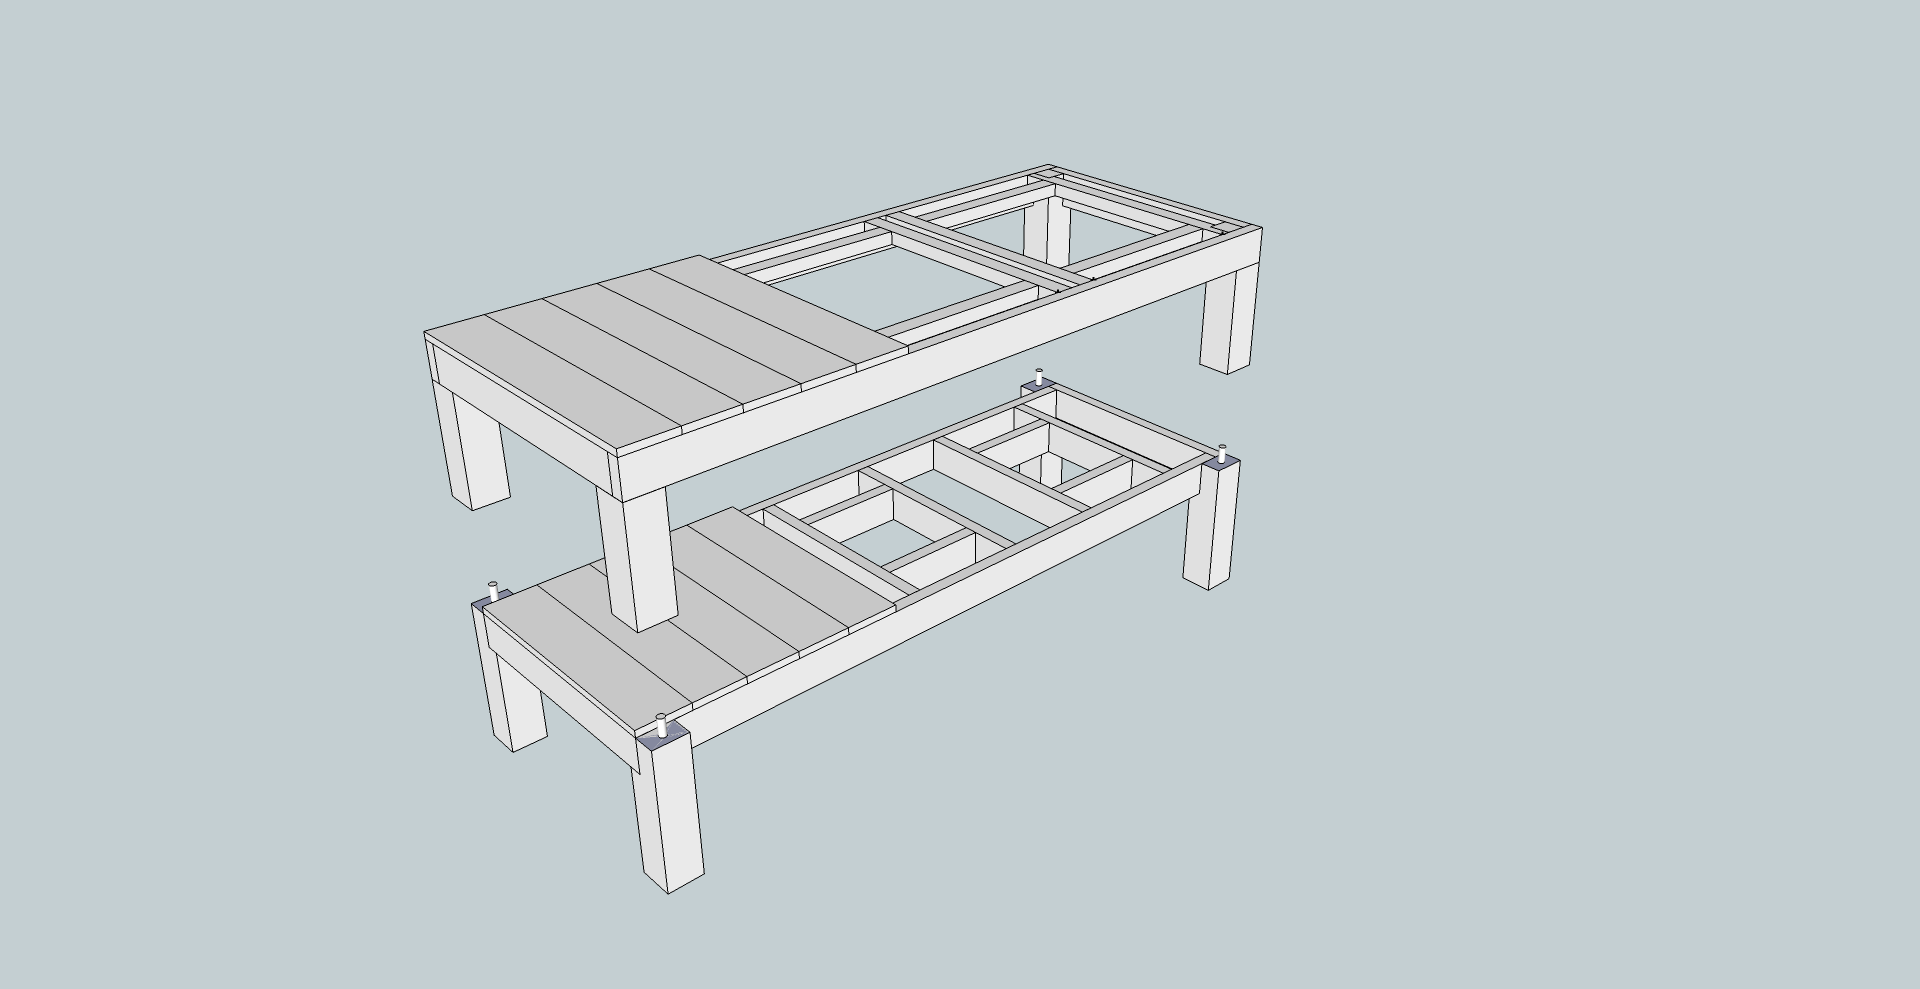
\includegraphics[scale=0.15]{bench_above}
\caption{Bench, above}
\label{bench_above}
\end{figure}

\begin{figure}[h]
\centering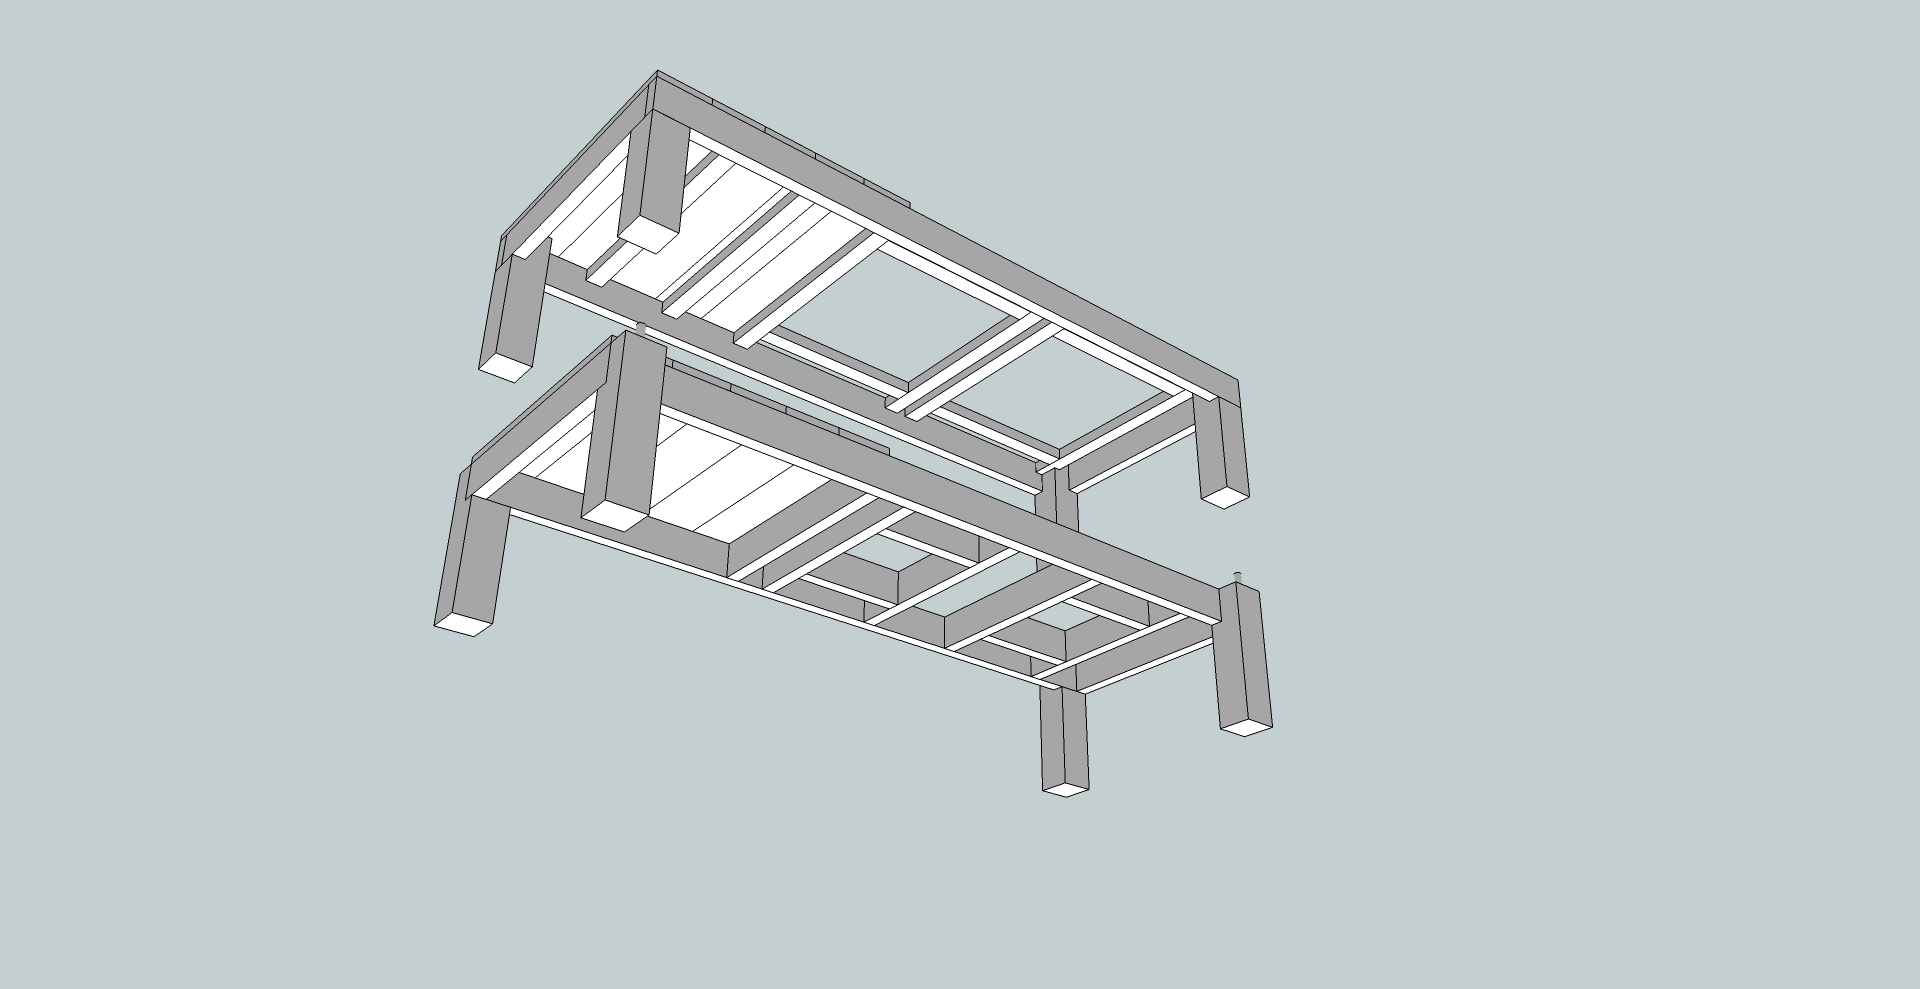
\includegraphics[scale=0.15]{bench_below}
\caption{Bench, below}
\end{figure}

\section{Sizes}

The bench is 80cm tall, 80cm deep and 200cm wide. The feet are cut 2x40cm long.

\section{Considerations}

\subsection{Transportation}

It should be easy to transport the bench. As it is very heavy, it is divided into two parts that each can be transported on the roof of a car. The parts of the bench will be assembled together using metal rods, according to figure \ref{bench_above}.

\subsection{Surface treatment}

The wood will have to be treated so that it can withstand spills of boiling wort.

%----------------------------------------------------------------------------------------

\chapterimage{metal.pdf} % Chapter heading image

\chapter{Metalworking}

\section{Tanks}

All tanks are made from OSO brand hot water tanks (1977-1990 model). These come with a 50mm threaded hole for a heating element. The bottom parts of the tanks have feet.

According to varius forum threads, these tanks are made of 4mm thick (measured) stainless steel, grade 304.

There are adapters available to reduce the 50mm hole to a standard 1" threaded hole.\\

The system is sized to accomodate brewing 120L of finished beer using 48kg of malt.

\subsection{HLT}

The HLT is cut for a volume of 130L.

It is the bottom part of an OSO brand tank and has one heating element and feet. A $1 \over 2$" hole is drilled in the bottom for draining water.  There is a $1 \over 2$" inlet on the side for return from the RIMS-tube.

\subsection{MLT}

The MLT is cut for a volume of 170L. 

It is the top part of an OSO brand tank and has no feet. The inlet on the side is plugged with a male, threaded pipe cap.

\subsection{BK}

The BK is cut for a volume of approximately 190L

It has feet and two heating elements. The second element is mounted as a weldless fitting.

\subsection{Initial cleaning}

The tanks are initially cleaned using diluted hydrochloric acid. This is then neutralized using dilute sodium bicarbonate to prevent the acid from etching the steel. The procedure efficiently removes calcium and iron salts.

Further cleaning is performed using soap and hot water.

\section{Welding}

A 4" sanitary ferrule is welded to the bottom of the mash / lauter tun and the boil kettle to aid in removal of spent grains and cleaning.

We only have access to a MIG welder, so every part will be welded using MIG. TIG is recommended for this kind of job but a MIG will also do fine (makes a somewhat sloppier seam).\\

Suggested welding parameters % ref http://www.howtobrew.com/appendices/appendixB-3.html

\begin{table}[ht!]
\centering
\begin{tabular}{l l l l l l l l}
\toprule
Method & Steel thickness & Current & Voltage & Weld wire & Argon flow & Weld speed & Wire feed\\ 
\toprule
 & mm & amp & volts & AWS spec & $m^3 \over h$ & $cm \over min$ & $cm \over min$\\
\midrule
MIG & 1.6 & 85 DCEP & 21 & ER316L & 0.42 & 48 & 467\\
TIG & 1.14 - 2.29 & 37 - 70 DCEN & 12 - 14 & ER316L & 0.34 & 5 - 10 & As req.\\
\bottomrule
\end{tabular}
\caption{Suggested welding parameters}
\end{table}

\section{Weldless fittings}

Holes are made using a step drill bit. All weldless fittings are threaded and mounted with an O-ring and nut.

\section{Chiller}

The chiller is a counter flow design with an inner copper tube of 6m length and an outer tube of PVC.

Copper wire is coiled around and soldered to the inner tube to generate turbulence in the water stream. Soap is used as lubricant to aid in inserting the inner tube into the PVC hose.

The PVC hose is connected to the tee using a hose barb. The inner tube is connected to the tee using compression fittings.

%----------------------------------------------------------------------------------------

\chapterimage{control.pdf} % Chapter heading image

\chapter{Control system}

\section{PCB's}

An inital attempt at placing all the components on a single PCB resulted in a messy PCB with lots of airwires. The circuit is therefore divided into three parts

\begin{itemize}
\item Mainboard, containing the Arduino, the USB interface and a programming header
\item Relay interface, containing optocouplers and screw terminals
\item Thermocouple interface, containing a voltage regulator, level switching, interface chips and screw terminals
\end{itemize}

\section{Relays}

The price difference of SSR's and mechanical relays is close to none, and as SSR's are quiet and require almost no addition electronics all the relays in this system are of solid state type.

The SSR's that are going to do power width modulation are of recognized brands. The SSR's that are used to only turn on and off i.e. the pump are of generic eBay brands.

\section{Sensors}

\subsection{Flow}

A flow sensor with a rating of 0-30 $L \over min$ is used to measure the volume of tap water in the HLT.

The flow rating of tap water in Trondheim, Norway is on average about 15 $L \over min$. The sensor is chosen closest to this rating as a sensor with a wider rating is thought to be less accurate.

\subsection{Temperature}

\subsubsection{Probes}

All probes are K-type thermocouples with a range of $0\degree$C \textasciitilde $400\degree$C.

\subsubsection{Interface chip}

The thermocouples are interfaced with MAX31855KASA chips.

\section{Computers and microcontrollers}

All sensors are connected to an ATMega328p programmed with the Arduino bootloader and the V-USB library. The ATMega328p then communicates over USB to a Raspberry Pi running Debian Linux. Communication by the user with the Raspberry Pi is performed over a standard ethernet LAN.

\subsection{5V to 3.3V level conversion}

The MAX31855KASA chips are operated at 3.3V, while the Arduino and SSR's will be operated at 5V. Level conversion is done by following Adafruits design of their MAX31855 breakout board.

A switching diode is placed wih the cathode connected to the output of the interface chip. The anode is connected to an input on the microcontroller. A resistor in series with a 3.3V supply is wired in parallel to this diode. When the microcontroller is outputting a digital zero, the anode of the diode is connected to ground and the path of shortest resistance from the interface chips input is ground. As the microcontroller outputs a digital one, the diode works as an off switch that disconnects the microcontroller and interface chip. The interface chip then gets fed 3.3V through the resistor.

According to the datasheet of the ATMega328p, the ''I/O pin input threshold voltage'' at $V_{cc} = 5V$ is about 2.6V. An input of 3.3V is therefore registered as a digital one.

%ref: http://www.atmel.com/Images/Atmel-8271-8-bit-AVR-Microcontroller-ATmega48A-48PA-88A-88PA-168A-168PA-328-328P_datasheet.pdf

\subsection{Schematic}

\begin{figure}[h]
\centering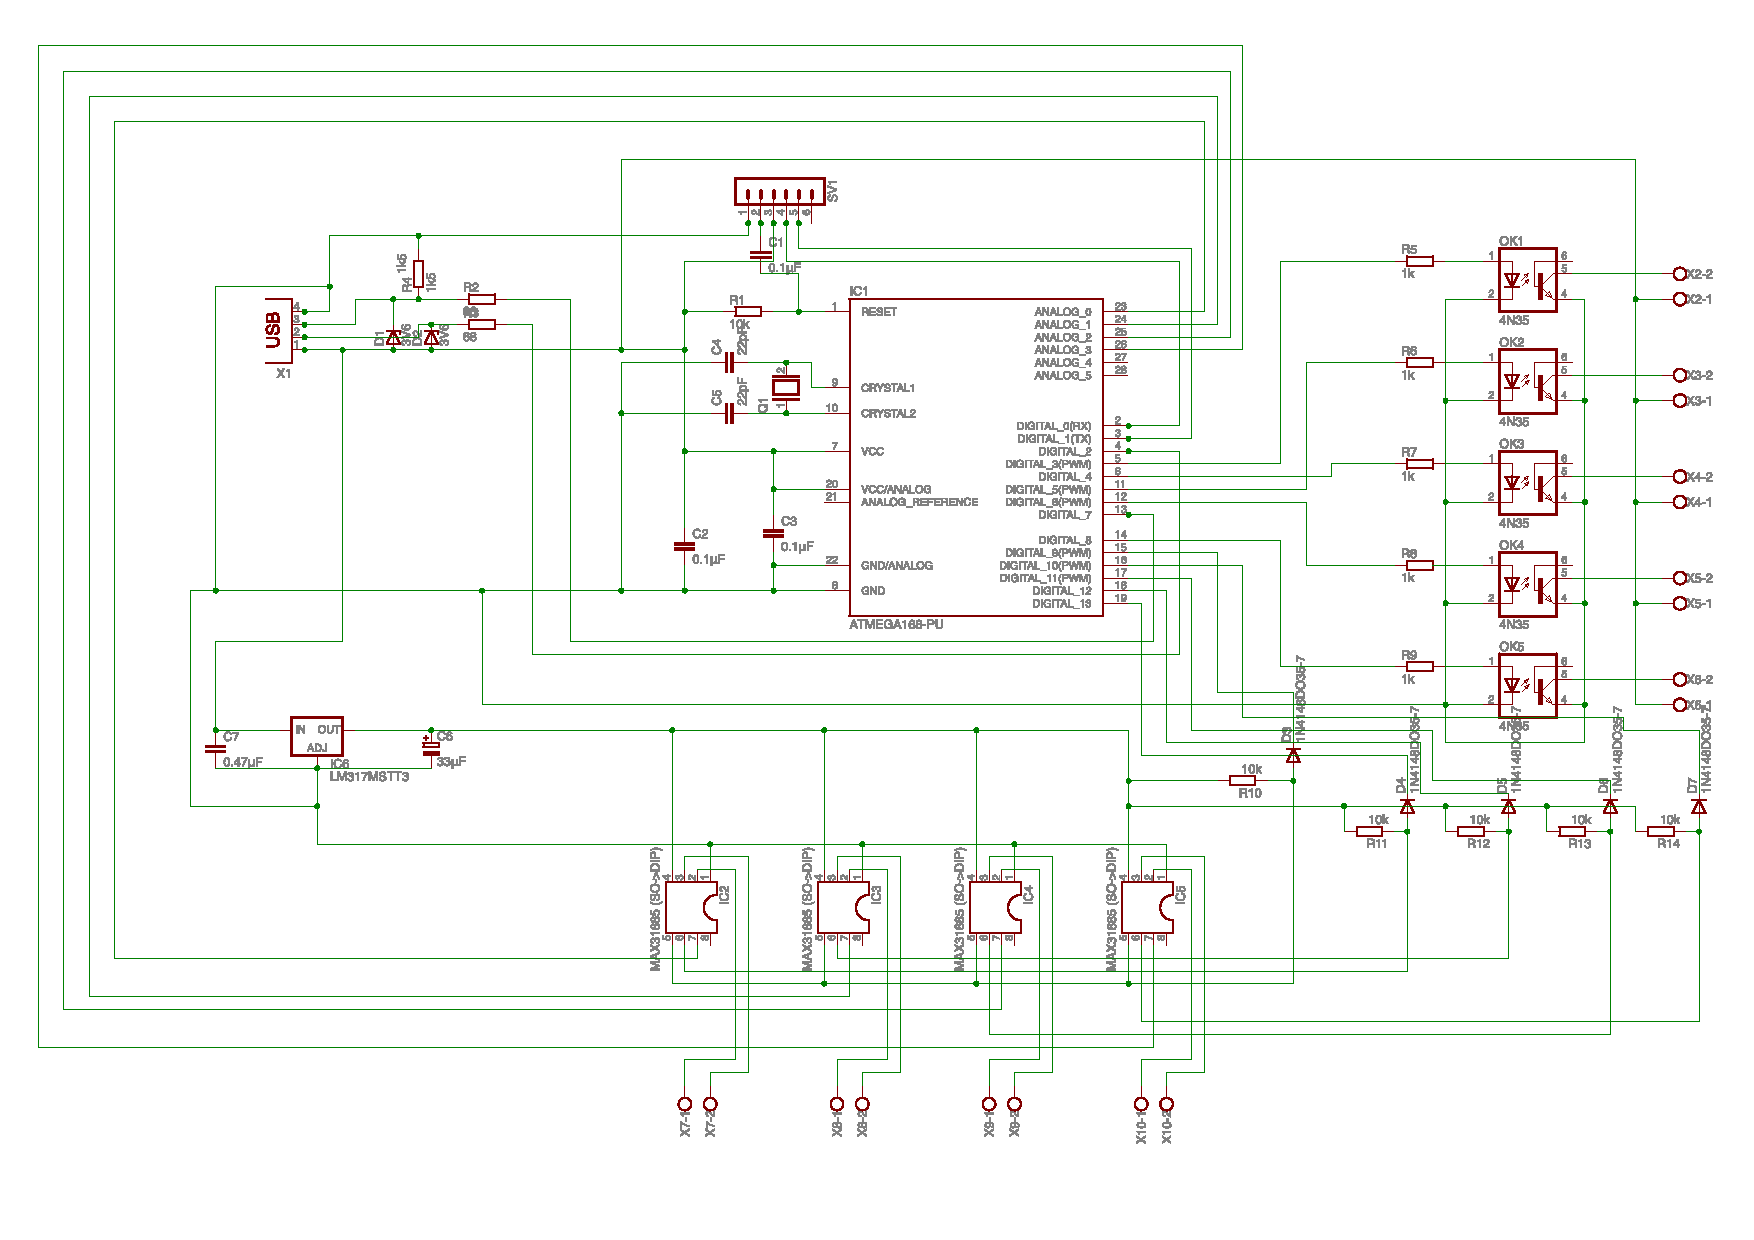
\includegraphics[scale=0.5]{mainboard_schem}
\caption{Schematic, mainboard}
\label{mainboard_schem}
\end{figure}


%----------------------------------------------------------------------------------------
%	PART 3
%----------------------------------------------------------------------------------------

\part{Bibliography and index}

%----------------------------------------------------------------------------------------
%	BIBLIOGRAPHY
%----------------------------------------------------------------------------------------

\chapterimage{chapter_head_1.pdf} % Chapter heading image

\chapter*{Bibliography}
\addcontentsline{toc}{chapter}{\textcolor{ocre}{Bibliography}}
\section*{Books}
\addcontentsline{toc}{section}{Books}
\printbibliography[heading=bibempty,type=book]
\section*{Articles}
\addcontentsline{toc}{section}{Articles}
\printbibliography[heading=bibempty,type=article]
\section*{Manuals}
\addcontentsline{toc}{section}{Manuals}
\printbibliography[heading=bibempty,type=manual]



%----------------------------------------------------------------------------------------
%	INDEX
%----------------------------------------------------------------------------------------

\cleardoublepage
\setlength{\columnsep}{0.75cm}
\addcontentsline{toc}{chapter}{\textcolor{ocre}{Index}}
\printindex

%----------------------------------------------------------------------------------------

\end{document}